\svnid{$Id$}
\chapter{Discussion and Completed Model}
\label{chap:completedmodel}
%Therefore I have integrated microbiological techniques with mathematical modelling principles to allow us to understand the system in a way previously not possible. I have constructed a mathematical model which describes \Nsm{} respiration \textit{in silico} and can produce predictions for the system \textit{in vivo}. To parameterise this model I used a novel integrative scheme where a standard Bayesian fitting methodology is interleaved with iterative experimental data collection on progressively more complex respiratory scenarios.
From Chapter \ref{chap:intro}, the stated aims of this thesis were:
\begin{enumerate}
\item {\bf Construct a mathematical model of the \Nm{} respiratory chain.} This will involve the conversion of the kinetic reactions involved in respiration into mathematical equations that can be linked together, and if justified simplifying the chain.
\item {\bf Obtain experimental data on respiratory rates and enzyme kinetics.} This will involve performing experiments on respiring \Nm{} and recording the concentrations of respiratory substrates under different conditions.
\item {\bf Parametrise the model using experimental data.} To do this a system will need to be developed which can iteratively fit experimental data to specific parts of the mathematical model.
\end{enumerate}

\noindent With reference to the above, a mathematical model was constructed as described in Chapter \ref{chap:model}, the equations shown below:
\begin{eqnarray*}
\frac{d[O_2]}{dt} & = & \beta(1-[O_2]/K_O) - k_{1}[C_a][O_2]\\ \nonumber
\frac{d[NO]}{dt} & = & m_{1}[NO_2^-][A_a] - l_1[NO][B_a] - k_5[C_a][NO] + k_6 [C_X] - \gamma[NO]\\ \nonumber
\frac{d[NO_2^-]}{dt} & = & - m_{1}[NO_2^-][A_a]\\ \nonumber
\frac{d[Q_a]}{dt} & = & g([Q] - [Q_a]) - l_3[Q_a]([B] - [B_a]) - f[Q_a]([X]-[X_a])\\ \nonumber
\frac{d[X_a]}{dt} & = & -k_3([C] - [C_a] - [C_X])[X_a]  - m_3([A] - [A_a])[X_a] + f[Q_a]([X]-[X_a])\\ \nonumber
\frac{d[C_a]}{dt} & = & k_3([C] - [C_a] - [C_X])[X_a] - k_{1}[C_a][O_2] - k_5[C_a][NO] + k_6[C_X]\\ \nonumber
\frac{d[C_X]}{dt} & = & k_5[C_a][NO] - k_6 [C_X]\\ \nonumber
\frac{d[A_a]}{dt} & = & m_3([A] - [A_a])[X_a]- m_{1}[NO_2^-][A_a]\\ \nonumber
\frac{d[B_a]}{dt} & = & l_3[Q_a]([B] - [B_a]) - l_1[NO][B_a]
\end{eqnarray*}
Additionally if the preliminary suggested expression equations are to be included this list is extended to include:
\begin{eqnarray*}
\frac{d[A]}{dt} & = & \left(R\left(1 - \frac{[O_2] + k_{10}[NO]}{[O_2] + k_{10}[NO] + k_{11}}\right) - S\left(1 - \frac{[NO]}{[NO] + k_{13}}\right)\right) - k_8[A] \nonumber \\
\frac{d[B]}{dt} & = & T \left(\frac{[NO]}{[NO] + k_{15}}\right) - k_{16}[B]
\end{eqnarray*}

The data required to populate the parameters has been obtained by experimental means as described in Chapters \ref{chap:oxygenreduction}-\ref{chap:nitritereduction}. These data provided information on both respiratory rates and enzymes kinetics. Additional information was gathered from the literature as shown in Chapter \ref{chap:model}.

To use the information obtained from the literature and from experimental data, an integrated parameter estimation scheme was devised, which combined Bayesian inference with a Monte-Carlo type parameter estimation system into an iterative method for extracting parameter values from progressively more complex datasets as described in Chapter \ref{chap:paramest}. This iterative method produces posterior probability distributions for each of the parameters in the model calculated from the various rounds of parameter estimation for each successive dataset. The final parameter probability distributions are shown in tabular form in Table \ref{tab:final_parameters}. This table shows the values required to produce idealised lognormal distributions of each of the parameters. Plots of the actual obtained distributions are shown in Figure \ref{fig:final_posteriors}.
\begin{table}[tbp]
\begin{center}
\begin{tabular}{>{\centering}m{1.4cm}>{\centering}m{6.1cm}>{\centering}m{2.7cm}>{\centering}m{2.5cm}}
\toprule
\textbf{Symbol} & \textbf{Description} & \textbf{Mean Value} & \textbf{$\sigma$}
\tabularnewline
\midrule
$k_1$ & Rate constant for O$_{\textrm{2}}$ reduction by reduced \cbbthree{} & $403.51~\mu M^{-1} s^{-1}$ & $27.59$
\tabularnewline\noalign{\smallskip}\hline\noalign{\smallskip}

$k_3$ & Rate constant for \cbbthree{} reduction by cytochrome pool & $4.58~\mu M^{-1} s^{-1}$ & $0.436$
\tabularnewline\noalign{\smallskip}\hline\noalign{\smallskip}

$l_1$ & Rate constant for NO reduction by reduced NorB & $6.42~\mu M^{-1} s^{-1}$ & 2.33
\tabularnewline\noalign{\smallskip}\hline\noalign{\smallskip}

$l_3$ & Rate constant for NorB reduction by quinone pool & $0.096~\mu M^{-1} s^{-1}$ & $0.025$
\tabularnewline\noalign{\smallskip}\hline\noalign{\smallskip}

$m_1$ & Rate constant for NO$_{\textrm{2}}^{\textrm{-}}$ reduction by reduced AniA & $0.175~\mu M^{-1} s^{-1}$ & $0.087$
\tabularnewline\noalign{\smallskip}\hline\noalign{\smallskip}

$m_3$ & Rate constant for AniA reduction by cytochrome pool & $4.79~\mu M^{-1}s^{-1}$ & $0.042$
\tabularnewline\noalign{\smallskip}\hline\noalign{\smallskip}

$k_5$ & Rate constant for \cbbthree{} inhibition by NO & $\approx66000~\mu M ^{-1} s ^{-1}$ & Indeterminate
\tabularnewline\noalign{\smallskip}\hline\noalign{\smallskip}

$k_6$ & Rate constant for recovery of NO inhibited \cbbthree{} & $1.59~s^{-1}$ & $0.527$
\tabularnewline\noalign{\smallskip}\hline\noalign{\smallskip}

$\beta$ & Rate constant for passive diffusion in of O$_{\textrm{2}}$ & $0.00014~\mu M^{-1} s^{-1}$ & $4.7\times10^6$
\tabularnewline\noalign{\smallskip}\hline\noalign{\smallskip}

$K_O$ & Saturation O$_{\textrm{2}}$ level & $48~\mu M$ & $0$
\tabularnewline\noalign{\smallskip}\hline\noalign{\smallskip}

$g$ & Rate of electrons in from NADH & $0.085~s^{-1}$ & $0.0078$
\tabularnewline\noalign{\smallskip}\hline\noalign{\smallskip}

$f$ & Rate constant for reduction of cytochromes by quinones & $0.771~\mu M^{-1}s^{-1}$ & $0.096$
\tabularnewline\noalign{\smallskip}\hline\noalign{\smallskip}

$\gamma$ & Spontaneous loss of NO & $0.0024~\mu Ms^{-1}$ & $8.8\times10^5$
\tabularnewline\noalign{\smallskip}\hline\noalign{\smallskip}

$Q$ & Concentration of quinones & $34.31~\mu M$ & $5.49$
\tabularnewline\noalign{\smallskip}\hline\noalign{\smallskip}

$X$ & Concentration of cytochromes & $2.81~\mu M$ & $0.595$
\tabularnewline\noalign{\smallskip}\hline\noalign{\smallskip}

$A$ & Concentration of AniA & $0.704~\mu M$ & $0.3$
\tabularnewline\noalign{\smallskip}\hline\noalign{\smallskip}

$B$ & Concentration of NorB & $7.8~\mu M$ & $3.63$
\tabularnewline\noalign{\smallskip}\hline\noalign{\smallskip}

$C$ & Concentration of \cbbthree{} & $1.3~\mu M$ & $0.259$
\tabularnewline
\bottomrule
\end{tabular}
\caption[Model parameters]{{\bf Model parameters.} This table shows all the parameter values that have been generated by iterative parameter estimation throughout this work. For values that show concentrations of components, they represent the value for a culture with $OD_{600}=1.00$.
\label{tab:final_parameters}}
\end{center}
\end{table}

\begin{figure}[tbp]
 \centering
 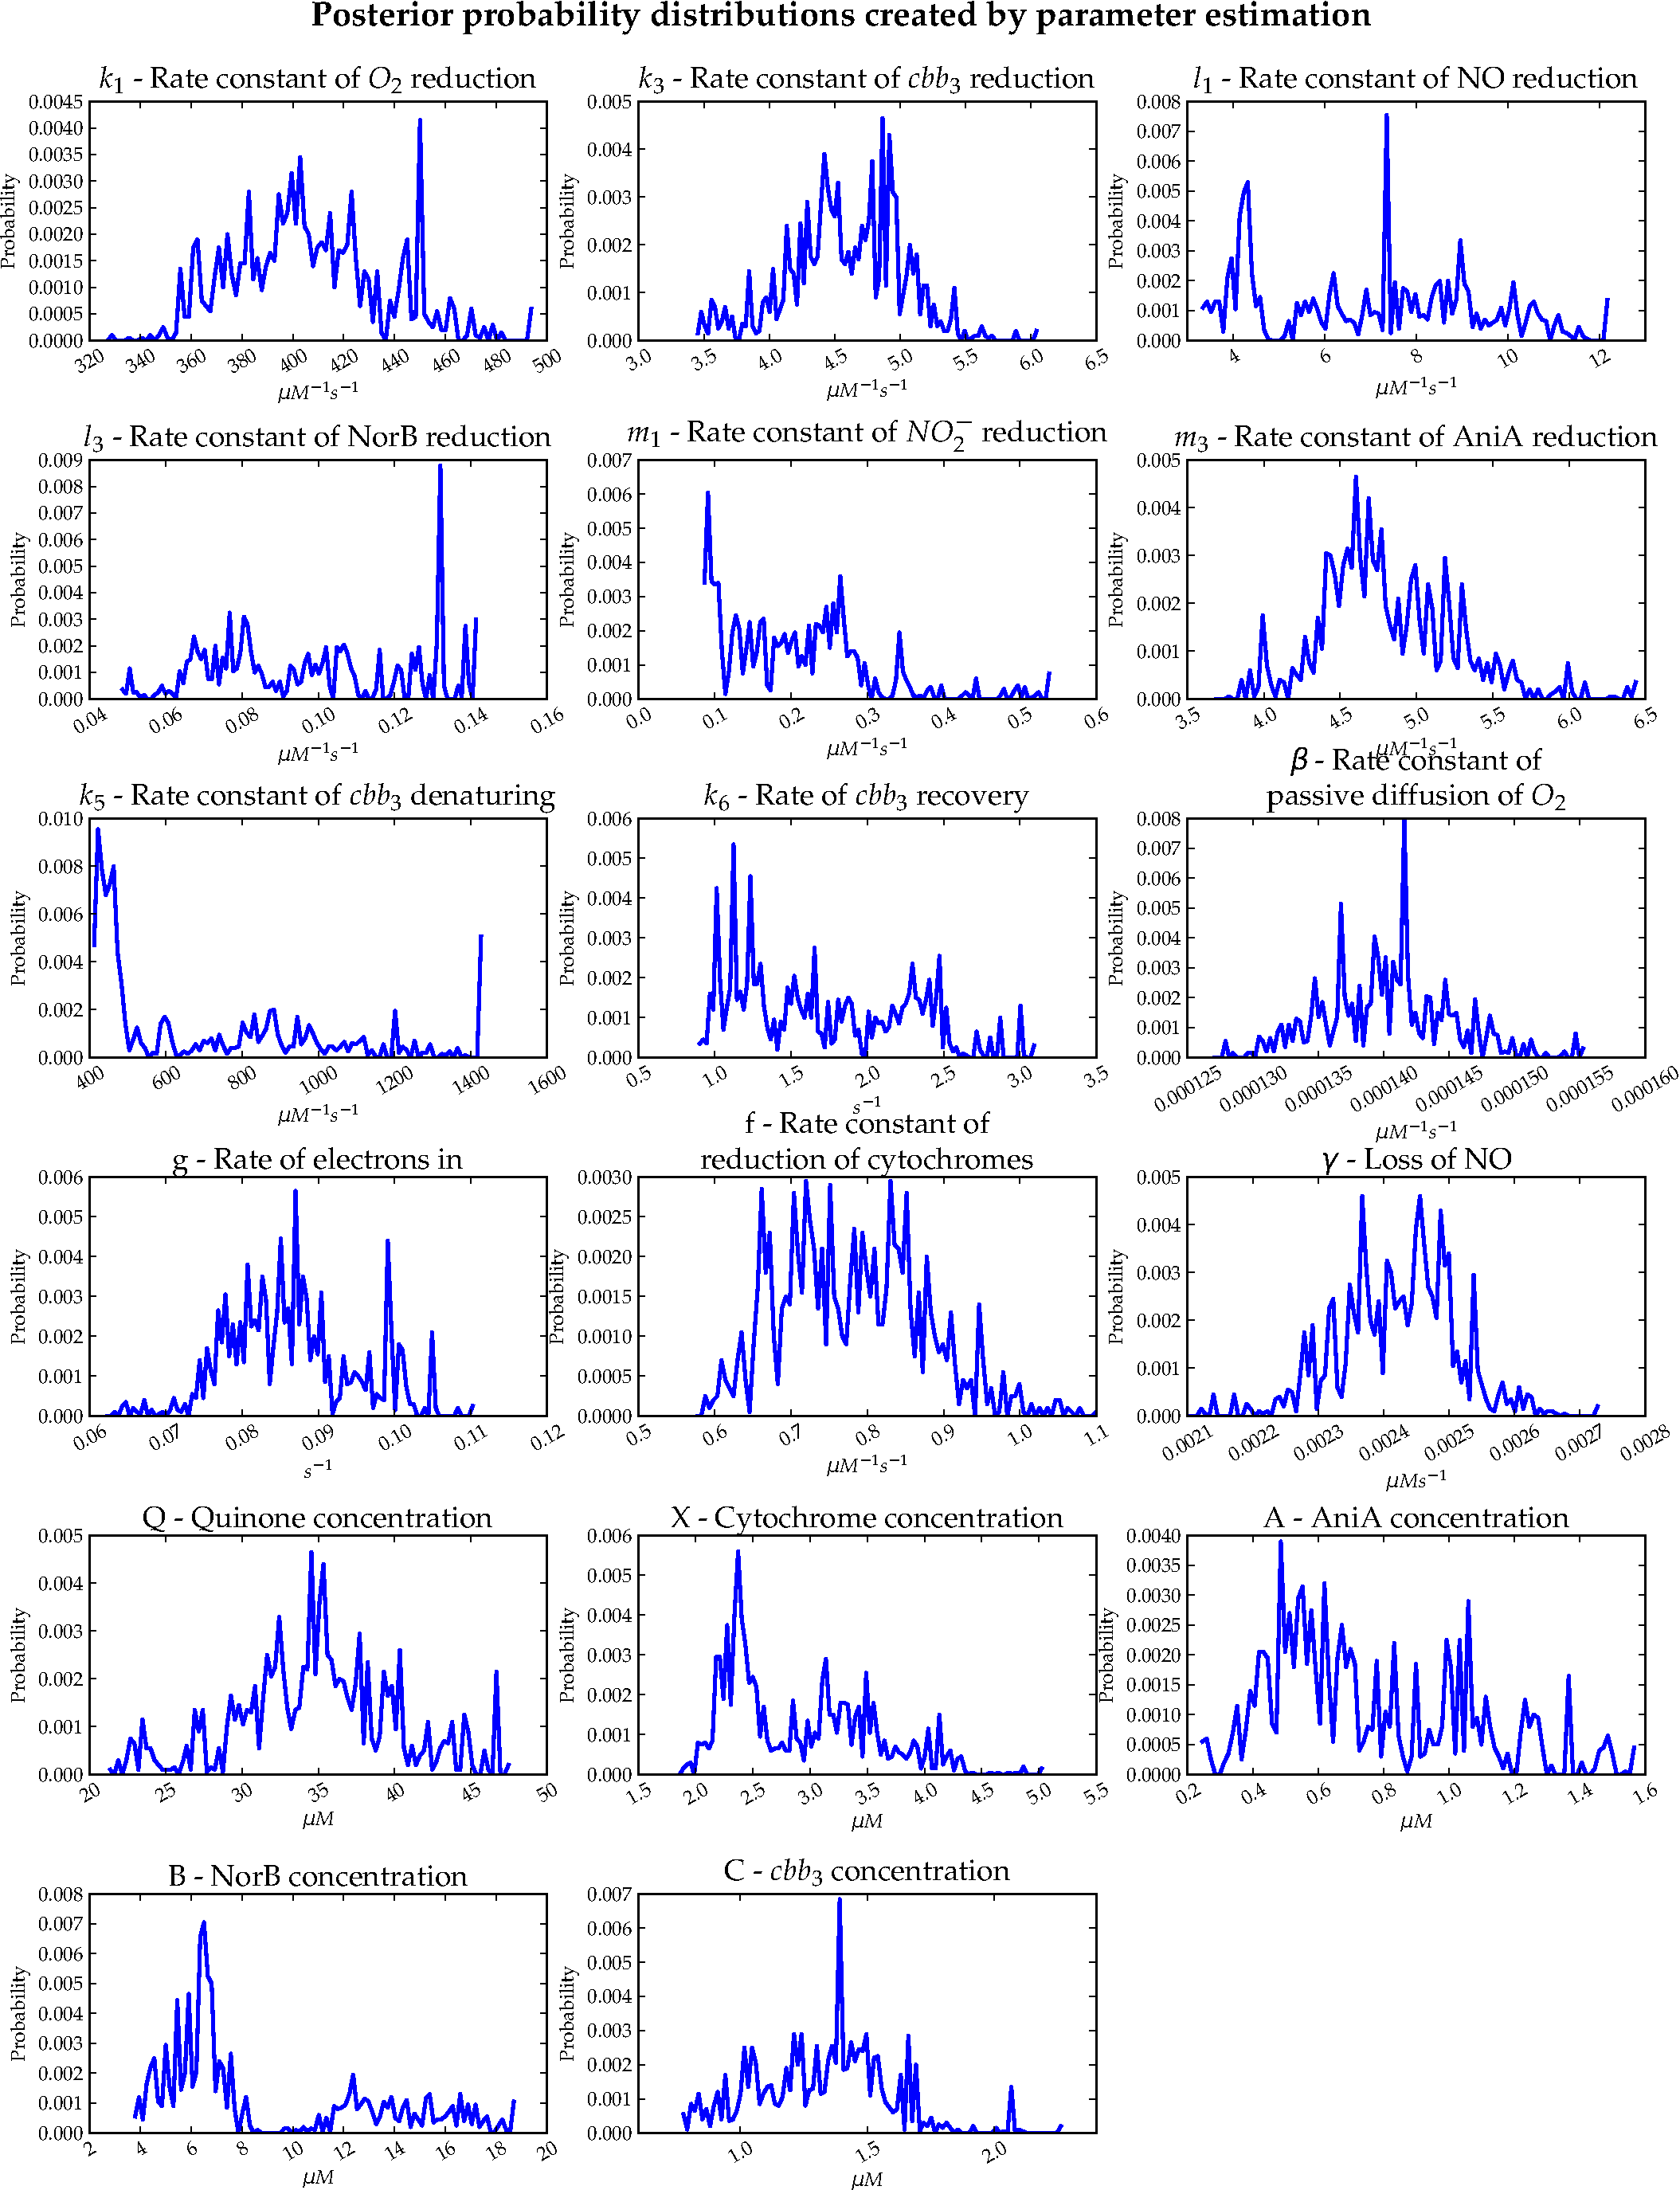
\includegraphics[width=15cm, trim=0cm 0cm 0cm 0cm, clip=true]{./09-completedmodel/data/posteriors.pdf}
 % priors.pdf: 1008x1008 pixel, 72dpi, 35.56x35.56 cm, bb=0 0 1008 1008
 \caption[Final Posterior probability distributions]{{\bf Final Posterior probability distributions}. These are the final posterior probability distributions generated by the parameter estimation system, all concentrations have been normalised to assume an $OD_{600}$ of 1. Note the value of $k_5$ will be significantly different from that shown.
 \label{fig:final_posteriors}}
\end{figure}

The value of $k_5$ has no associated bounds in the table as it was concluded that the value reported is actually much lower than the true value as evidenced in Chapter \ref{chap:nitritereduction} whereby the posterior parameters from nitrite reduction were unable to model the true effect of NO inhibition of oxygen shown in Chapter \ref{chap:noreduction}. Increasing the value of $k_5$ could restore the correct behaviour in the NO reduction dataset without a significant detrimental effect on the nitrite dataset. Unfortunately this makes the bounds on this value indeterminate without further Monte-Carlo simulation being run with the adapted value. The distribution shown in Figure \ref{fig:final_posteriors} shows the un-adapted values for comparison.

\section{Amalgamation of Cytochromes}
The choice to replace the multiple cytochromes $bc_1$, $c_x$, $c_4$ and $c_5$ with one single entity was a modelling one, to both simplify the modelling process by reducing the total component count and number of rate constants, and to allow the model to focus on simple electron transport chain branching and competition for electrons. The rate constants for each of the cytochromes could be subsumed by the respective ``out rates'' from the amalgamated cytochrome to its downstream electron acceptor. The downside of this approach is that it means that any rates obtained for $X$ are probably not going to be biologically relevant as it is essentially masking the behaviour of multiple different hidden components. This simplification does not appear to have affected the model in a detrimental way when using the datasets in this work.

\section{Parameter Changes Throughout this Work}
\begin{table}[tbp]
\begin{center}
\begin{tabular}{ccccc}
\toprule
\textbf{Parameter} & \textbf{Prior} & \textbf{Oxygen Posterior} & \textbf{NO Posterior} & \textbf{Nitrite Posterior}
\tabularnewline
\midrule
$k_1$ & $415$ & $413.228$ & $417.88$ & $403.51$
\tabularnewline\noalign{\smallskip}\hline\noalign{\smallskip}

$k_3$ & $3$ & $4.496$ & $4.65$ & $4.5$
\tabularnewline\noalign{\smallskip}\hline\noalign{\smallskip}

$l_1$ & $6$ & $\rightarrow$ & $13.12$ & $6.42$
\tabularnewline\noalign{\smallskip}\hline\noalign{\smallskip}

$l_3$ & $1$ & $\rightarrow$ & $0.058$ & $0.096$
\tabularnewline\noalign{\smallskip}\hline\noalign{\smallskip}

$m_1$ & $1$ & $\rightarrow$ & $\rightarrow$ & $0.175$
\tabularnewline\noalign{\smallskip}\hline\noalign{\smallskip}

$m_3$ & $4.8$ & $\rightarrow$ & $\rightarrow$ & $4.79$
\tabularnewline\noalign{\smallskip}\hline\noalign{\smallskip}

$k_5$ & $100$ & $\rightarrow$ & $1741.8$ & $66000$
\tabularnewline\noalign{\smallskip}\hline\noalign{\smallskip}

$k_6$ & $38$ & $\rightarrow$ & $1.076$ & $1.59$
\tabularnewline\noalign{\smallskip}\hline\noalign{\smallskip}

$\beta$ & $0.00014$ & $0.00012$ & $0.00014$ & $0.00014$
\tabularnewline\noalign{\smallskip}\hline\noalign{\smallskip}

$g$ & $0.847$ & $0.889$ & $0.857$ & $0.085$
\tabularnewline\noalign{\smallskip}\hline\noalign{\smallskip}

$f$ & $8.749$ & $8.707$ & $8.398$ & $0.771$
\tabularnewline\noalign{\smallskip}\hline\noalign{\smallskip}

$\gamma$ & $0.017$ & $\rightarrow$ & $0.0024$ & $0.0024$
\tabularnewline\noalign{\smallskip}\hline\noalign{\smallskip}

$Q$ & $0.3$ & $3.143$ & $7.06$ & $34.31$
\tabularnewline\noalign{\smallskip}\hline\noalign{\smallskip}

$X$ & $3.97$ & $4.732$ & $27.45$ & $2.81$
\tabularnewline\noalign{\smallskip}\hline\noalign{\smallskip}

$A$ & $0.137$ & $\rightarrow$ & $\rightarrow$ & $0.704$
\tabularnewline\noalign{\smallskip}\hline\noalign{\smallskip}

$B$ & $0.043$ & $\rightarrow$ & $0.137$ & $7.8$
\tabularnewline\noalign{\smallskip}\hline\noalign{\smallskip}

$C$ & $0.03$ & $0.043$ & $0.071$ & $1.3$
\tabularnewline
\bottomrule
\end{tabular}
\caption[Change in Parameter Values]{{\bf Change in Parameter Values.} This table shows the mean of each parameter value at each stage of the model. Where parameters are not used and therefore generate no posterior distribution, a $\rightarrow$ is used instead.
\label{tab:parameter_changes}}
\end{center}
\end{table}

The way the parameters change throughout the various rounds of parameter estimation described in this work is presented in Table \ref{tab:parameter_changes} and discussed below.
\begin{itemize}
\setlength{\itemsep}{0cm}
 \item $k_1$ - Changes very little and the final distribution resembles the prior distribution very closely.
 \item $k_3$ - Increases slightly to achieve the required oxygen reduction rate and affinity.
 \item $l_1$ - Increases by a factor of two initially however this is a very broad distribution suggesting that the magnitude is less important at this point. It settles back to a value closer to the prior when a more appropriate dataset is used.
 \item $l_3$ - Reduces significantly to achieve desired NO reduction rate.
 \item $m_1$ - Reduces significantly to achieve desired nitrite reduction rate.
 \item $m_3$ - Changes very little from prior distribution.
 \item $k_5$ - Increases significantly in order to inhibit \cbbthree{} by the amount seen in experimental data.
 \item $k_6$ - Decreases significantly for the same reason as above.
 \item $\beta$ - No change.
 \item $g$ - No change initially, but final posterior shows a $10\times$ decrease to prevent permanent reduction of cytochromes.
 \item $f$ - No change initially, but final posterior shows a $10\times$ decrease to prevent permanent reduction of quinone pool.
 \item $\gamma$ - Initial decrease to prevent NO being lost too quickly from the \textit{in silico} results.
 \item $Q$ - Initial increase to allow enough electron flux through the system. Final large increase as a result of reducing electron flux \textit{into} the system.
 \item $X$ - Significant change seen for NO reduction, but this change is negated in the final posteriors after reducing electron flux.
 \item $A$ - Significant increase required to attain observed Nitrite reduction rate after reducing electron flux.
 \item $B$ - Increases required to attain Nitric Oxide reduction rate, and after reducing electron flux.
 \item $C$ - Significant increase required to attain Oxygen reduction rate, exacerbated by the reduction of electron flux.
\end{itemize}

\section{Testing the Model}
\subsection{\texorpdfstring{Addition of Nitric Oxide to an \textit{nsrR}$^-$ mutant}{Addition of Nitric Oxide to an nsrR- mutant}}
The $nsrR^-$ mutant should express NorB at significantly higher levels than in wild-type cultures, by as much as $100\times$ according to \citet{Rock2007}. This is a simple \textit{in silico} test to do as it simple requires the concentration of NorB to be increased by $100\times$. Additionally a representative experimental dataset which has not been used during parameter estimation can be used to compare the \textit{in silico} result with the \textit{in vivo} data. This experimental dataset is shown in Figure \ref{fig:aniAnsrR} and repeated here in Figure \ref{fig:aniAnsrR1}.
\begin{figure}[tbp]
 \centering
 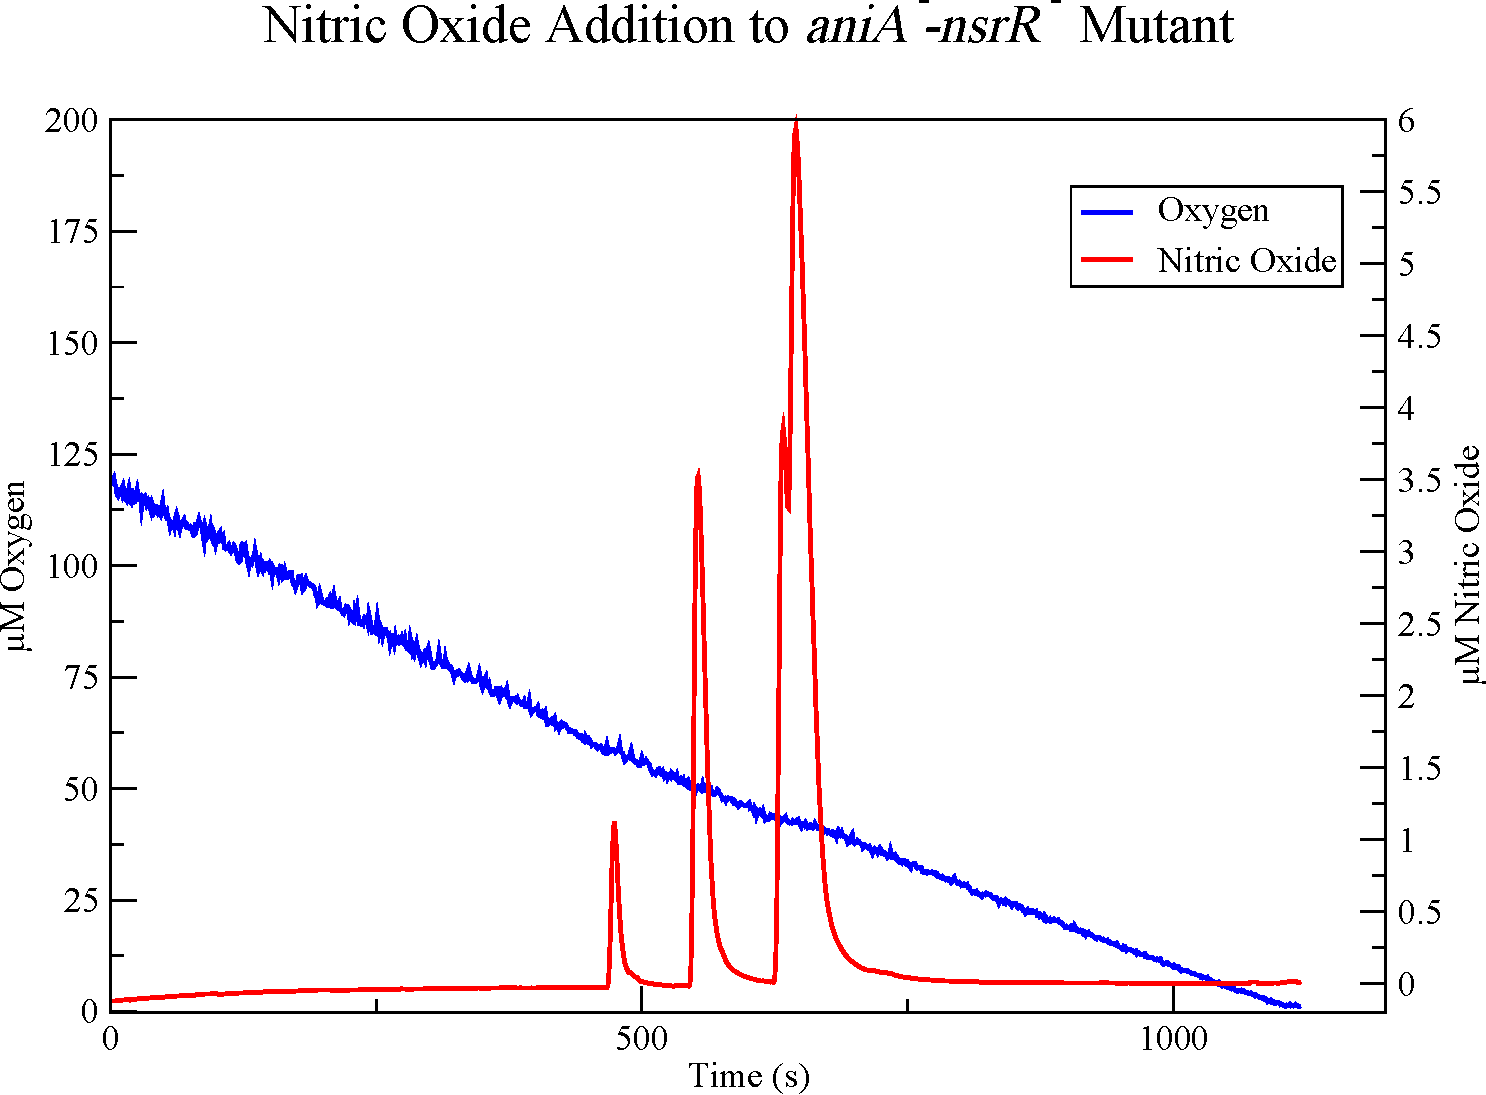
\includegraphics[width=15cm, clip=true]{./09-completedmodel/data/aniA-nsrR.pdf}
 % nosim.eps: 0x0 pixel, 300dpi, 0.00x0.00 cm, bb=0 0 794 595
 \caption[{Nitric Oxide Reduction in an nsrR Mutant.}]{{\bf Nitric Oxide Reduction in an $\mathbf{nsrR}^-$ Mutant.} This figure shows nitric oxide and oxygen reduction in an $aniA^-nsrR^-$. mutant. In this case the $aniA^-$ mutation has no effect as no nitrite is being reduced. Addition of nitric oxide has only a very small effect on the rate of oxygen reduction as it is being removed very quickly by the constitutively expressed NorB.}
 \label{fig:aniAnsrR1}
\end{figure}
The \textit{in silico} test was performed using the same parameter values used to generate Figure \ref{fig:nitric_oxide_simulation} with the value for NorB increased by $100\times$. The result of this simulation is shown in Figure \ref{fig:in_silico_nsrR}.
\begin{figure}[tbp]
 \centering
 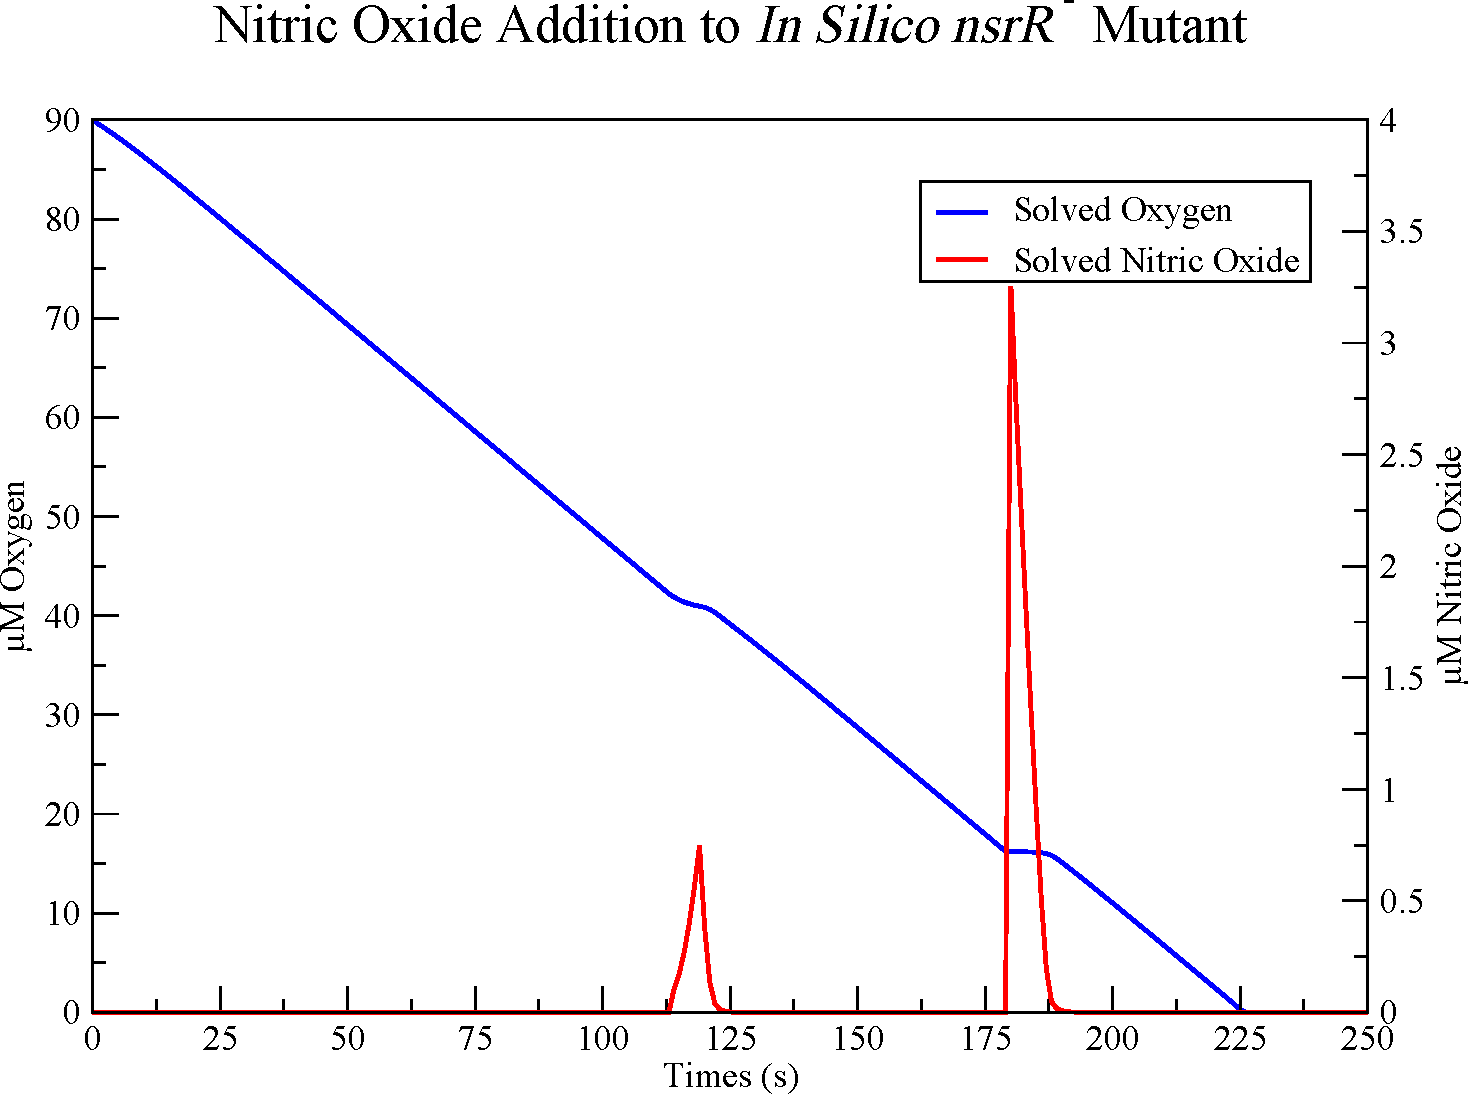
\includegraphics[width=15cm, clip=true]{./09-completedmodel/data/in_silico_nsrR.pdf}
 % in_silico_nsrR.pdf: 705x525 pixel, 72dpi, 24.87x18.52 cm, bb=0 0 705 525
 \caption[Nitric Oxide Addition to In silico nsrR Mutant]{{\bf Nitric Oxide Addition to \textit{In silico nsrR}$^-$ Mutant}. This figure shows the effect of adding two aliquots of increasing concentration of nitric oxide to a simulated $nsrR^-$ mutant.
 \label{fig:in_silico_nsrR}}
\end{figure}
This figure shows significant similarity with the experimentally observed result capturing the fast removal of nitric oxide due to the large quantities of NorB, and also models the slight reduction in oxygen reduction rate whilst the NO is being removed.

\subsection{\textit{In silico} cyt Knockouts}
It is possible to predict the effect on both the electron transport chain and the rates of respiration of knocking out some of the cytochromes that are encompassed within parameter $X$. This can be done by simply reducing the concentration of $X$ and leaving all other parameters unchanged. In this case the concentration was reduced by 25\% (this value is somewhat arbitrary but might be similar in effect knocking out 1 of the c-type cytochromes). This is a simplification of actually knocking out a specific cytochrome as this will actually affect all components downstream of $X$.

The experimental dataset used for comparison is that in Figure \ref{fig:nitrite_ds2_solved2}. The result of the simulated dataset is shown in Figure \ref{fig:in_silico_cyt} compared to the solved result from the wild-type.
\begin{figure}[tbp]
 \centering
 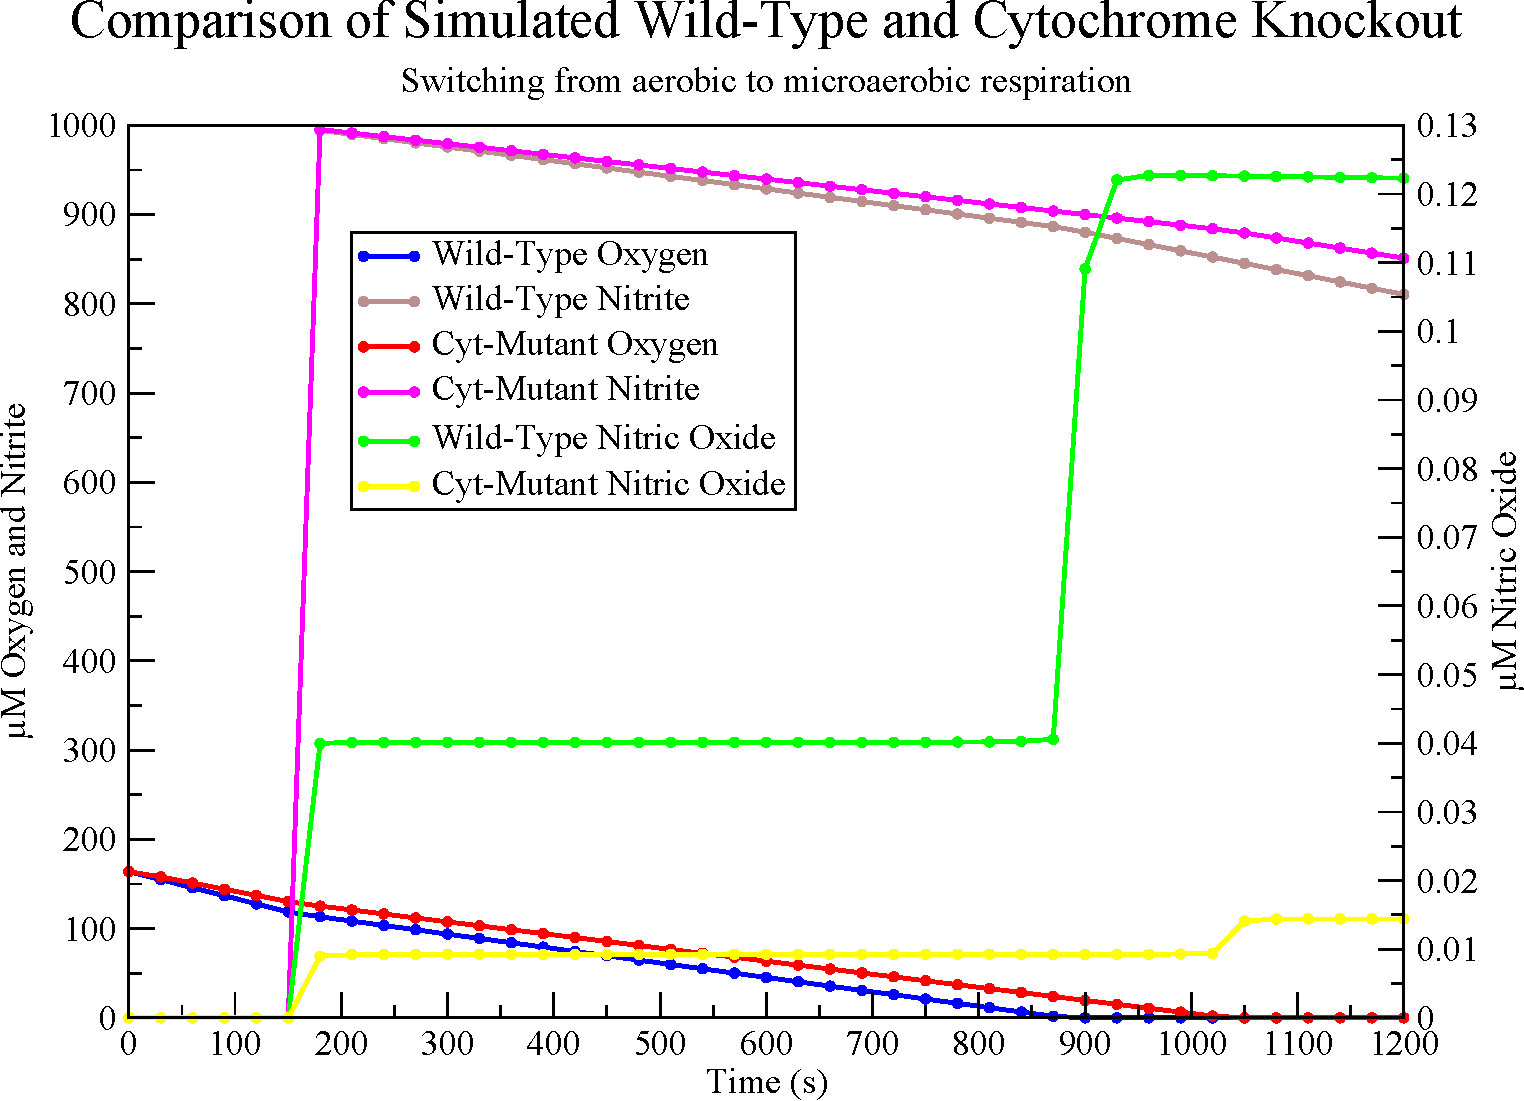
\includegraphics[width=15cm, clip=true]{./09-completedmodel/data/in_silico_cyt.pdf}
 % in_silico_nsrR.pdf: 705x525 pixel, 72dpi, 24.87x18.52 cm, bb=0 0 705 525
 \caption[In Silico Cytochrome Mutant]{{\bf \textit{In silico} Cytochrome Mutant}. This figure shows the effect of reducing the total amount of cytochromes while leaving all other components unchanged. All the reaction rates have slowed as a result of this change.
 \label{fig:in_silico_cyt}}
\end{figure}

The simulated cytochrome mutant shows that all reaction rates have slowed, although not by large amounts. The most obvious difference in the figure is the change in nitric oxide production and removal which is reduced to approximately 10\% of its production compared to the wild-type. This predicted result could easily be tested with an experiment using a c-type cytochrome knockout mutant grown in microaerobic conditions.

The reduction state plot can be seen in Figure \ref{fig:in_silico_cyt_redox}. It also compares the simulated cytochrome mutant to the wild-type. As can be seen, the redox states of \cbbthree{} and AniA do not change significantly as they are very efficient electron donors, remaining in an oxidised state. NorB remains in a more reduced state in the cytochrome mutant as there is less NO to ultimately reduce resulting in fewer electrons donated. The reduction state of the quinones is quite similar between the two simulations throughout. The reduction state of the cytochromes is significantly different, being higher than the wild-type at all times. This can be explained by looking at the quinone pool reduction state. As it remains fairly similar to the wild-type, the same flux of electrons must be passing through it, thus the same amount of electrons are being passed to fewer cytochromes. Since the rate of donation of electrons by the cytochromes has not been altered, the electrons build up in the cytochromes 
until a new steady-state is reached where the overall reduction state of the cytochromes is higher.

\begin{figure}[tbp]
 \centering
 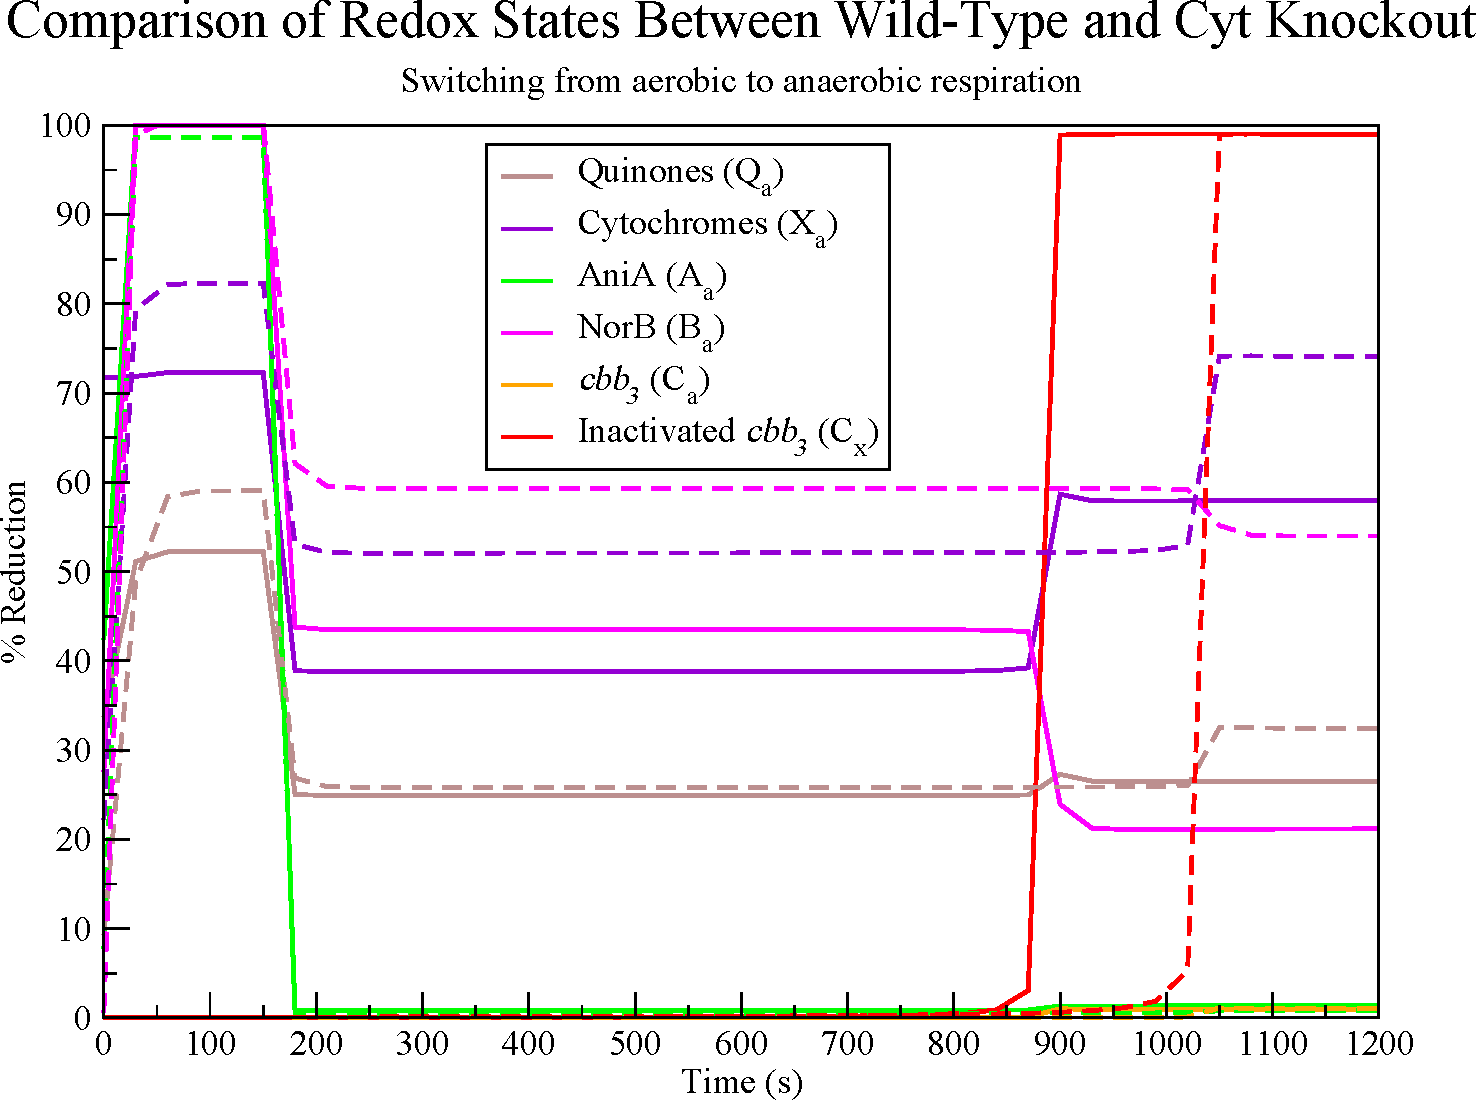
\includegraphics[width=15cm, clip=true]{./09-completedmodel/data/in_silico_cyt_redox.pdf}
 % in_silico_nsrR.pdf: 705x525 pixel, 72dpi, 24.87x18.52 cm, bb=0 0 705 525
 \caption[In Silico Cytochrome Mutant Redox States]{{\bf \textit{In silico} Cytochrome Mutant Redox States}. This figure shows the effect on the enzymatic reduction states of reducing the total number of cytochromes to simulate a cytochrome knockout mutant. The wild-type is represented by solid lines, and the synthetic mutant by dashed lines.
 \label{fig:in_silico_cyt_redox}}
\end{figure}

% \subsection{Electron Flux}
%
% \begin{eqnarray*}
% \mathrm{NADH~to~Quinone~rate~from~FBA} & = & 0.0173~Moles\cdot g^{-1}h^{-1}\\
% \times~2.8\times 10^{-13} g\cdot cell^{-1} & = & 4.844\times 10^{-15}~Moles\cdot cell^{-1}h^{-1}\\
% \div~3600~s\cdot h^{-1} & = & 1.35\times 10^{-18}~Moles\cdot cell^{-1}s^{-1}\\
% \div~1\times 10^{-15}~l\cdot cell^{-1} & = & 1.35\times 10^{-3} M\cdot s^{-1}\\
% \div~83\times 10^{-6}M & = & 16.3~s^{-1}
% \end{eqnarray*}

\section{Single Parameter Scaling Fits}
As has been discussed previously the proxy being used to try and estimate cell density appears to be inadequate as it does not scale correctly with the normalised data. It is however possible to obtain very good fits to all the experimental datasets with the exception of nitrite dataset 1 -  which is an $nsrR^-$ mutant - by simply introducing a ``scale factor'' which is applied to all concentrations in the system. An example of the better fit after using the scale factor is shown in Figure \ref{fig:improved_fit} in comparison to Figure \ref{fig:nitric_oxide_simulation}.

\begin{figure}[tbp]
 \centering
 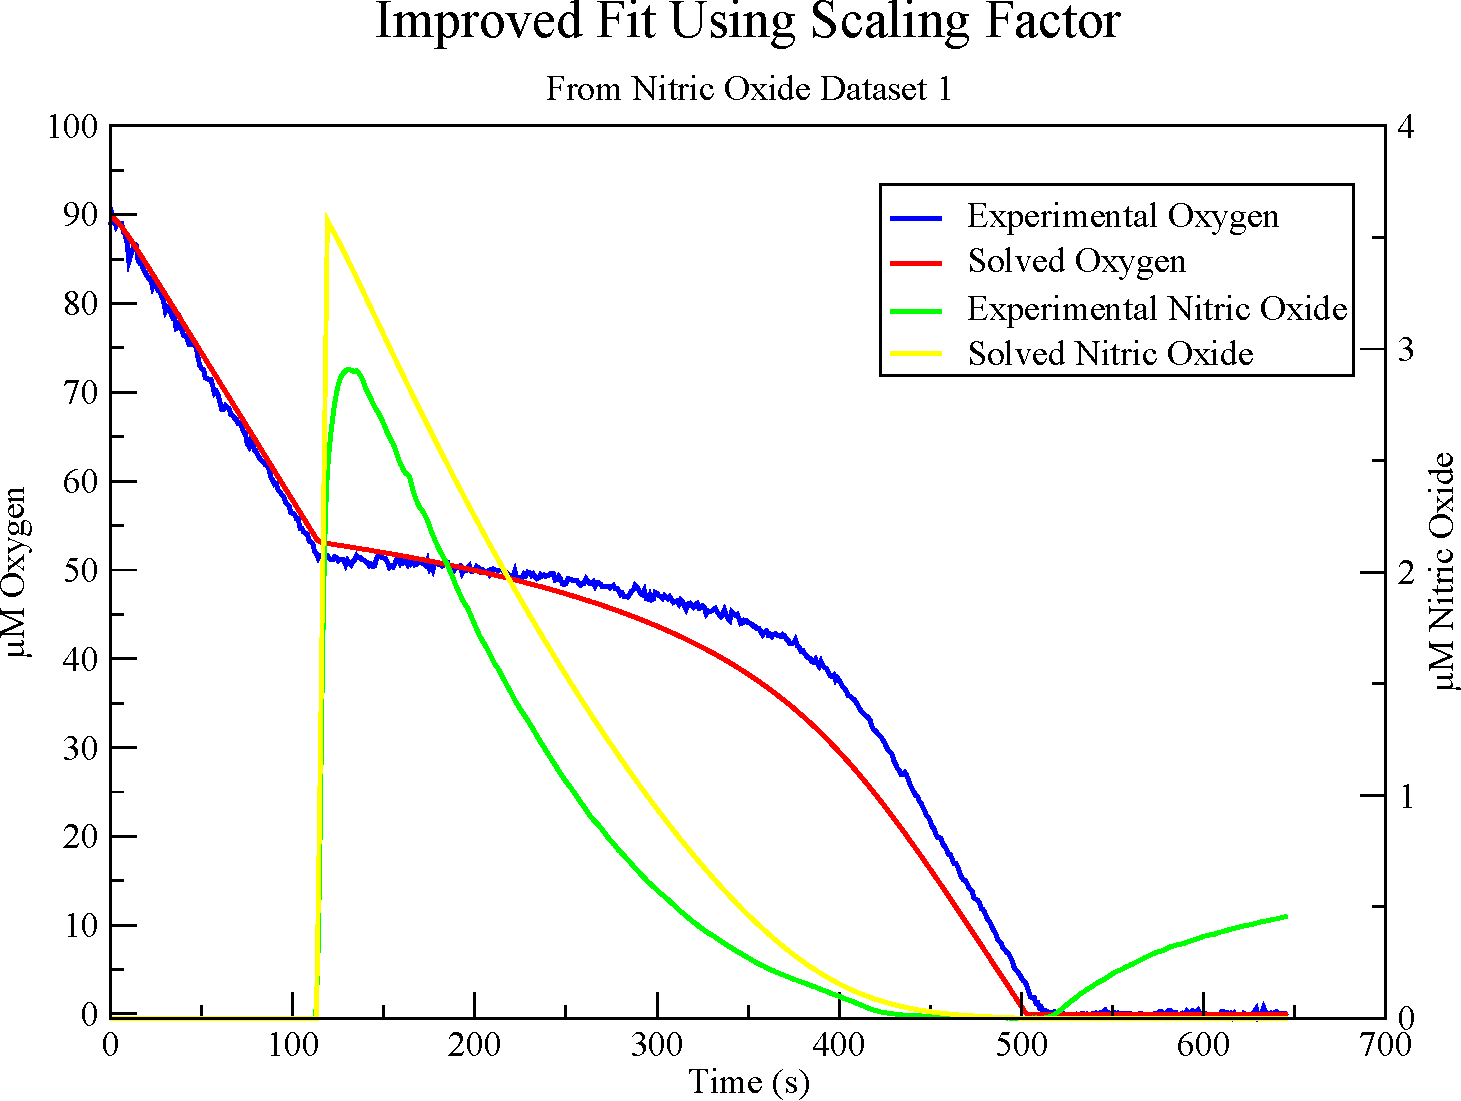
\includegraphics[width=15cm, clip=true]{./09-completedmodel/data/improved_fit.pdf}
 % in_silico_nsrR.pdf: 705x525 pixel, 72dpi, 24.87x18.52 cm, bb=0 0 705 525
 \caption[Improved Fit with Scaling Factor]{{\bf Improved Fit with Scaling Factor}. This figure shows the best fit achieved using a scaling factor rather than an approximate OD to calculate component concentrations. Compare with \ref{fig:nitric_oxide_simulation}.
 \label{fig:improved_fit}}
\end{figure}

The magnitude of the scale factor required for each dataset is shown in Table \ref{tab:scale-factors} along with the Oxygen Reduction Activity which formed part of the initial scaling.

\begin{table}[!ht]
\begin{center}
\begin{tabular}{ccc}
\toprule
Dataset & Scale Factor & $O_2$ Reduction Activity ($\mu Ms^{-1}$) \\
\midrule
Oxygen Dataset 1 & $\frac{1}{7}$ & 0.211027\\
\noalign{\smallskip}
Oxygen Dataset 2 & $\frac{1}{2.4}$ & 1.016159\\
\noalign{\smallskip}
Oxygen Dataset 3 & $\frac{1}{8}$ & 0.181488\\
\noalign{\smallskip}
Nitric Oxide Dataset 1 & $\frac{1}{5.5}$ & 0.336669\\
\noalign{\smallskip}
Nitric Oxide Dataset 3 & $\frac{1}{3}$ & 0.597478\\
\noalign{\smallskip}
Nitric Oxide Dataset 4 & $\frac{1}{5.8}$ & 0.324286\\
\noalign{\smallskip}
Nitrite Dataset 2 & $\frac{1}{5.8}$ (NorB $\frac{1}{5}$) & 0.275\\
\noalign{\smallskip}
\bottomrule
\end{tabular}
\end{center}
\caption{Dataset Scale Factors
\label{tab:scale-factors}}
\end{table}

The fact that NorB needed to be scaled by a smaller amount in Nitrite dataset 2 suggests that the value for NorB is actually underestimated in the priors. This does not affect the other datasets as they either have no NorB or only very low levels.

A plot of the scaling factors compared to the dataset oxygen reduction rates is shown in Figure \ref{fig:scaling-factors}. A simple linear regression through the datapoints suggests that the relationship between the two is approximately linear with a gradient of $0.36366$.

\begin{figure}[tbp]
 \centering
 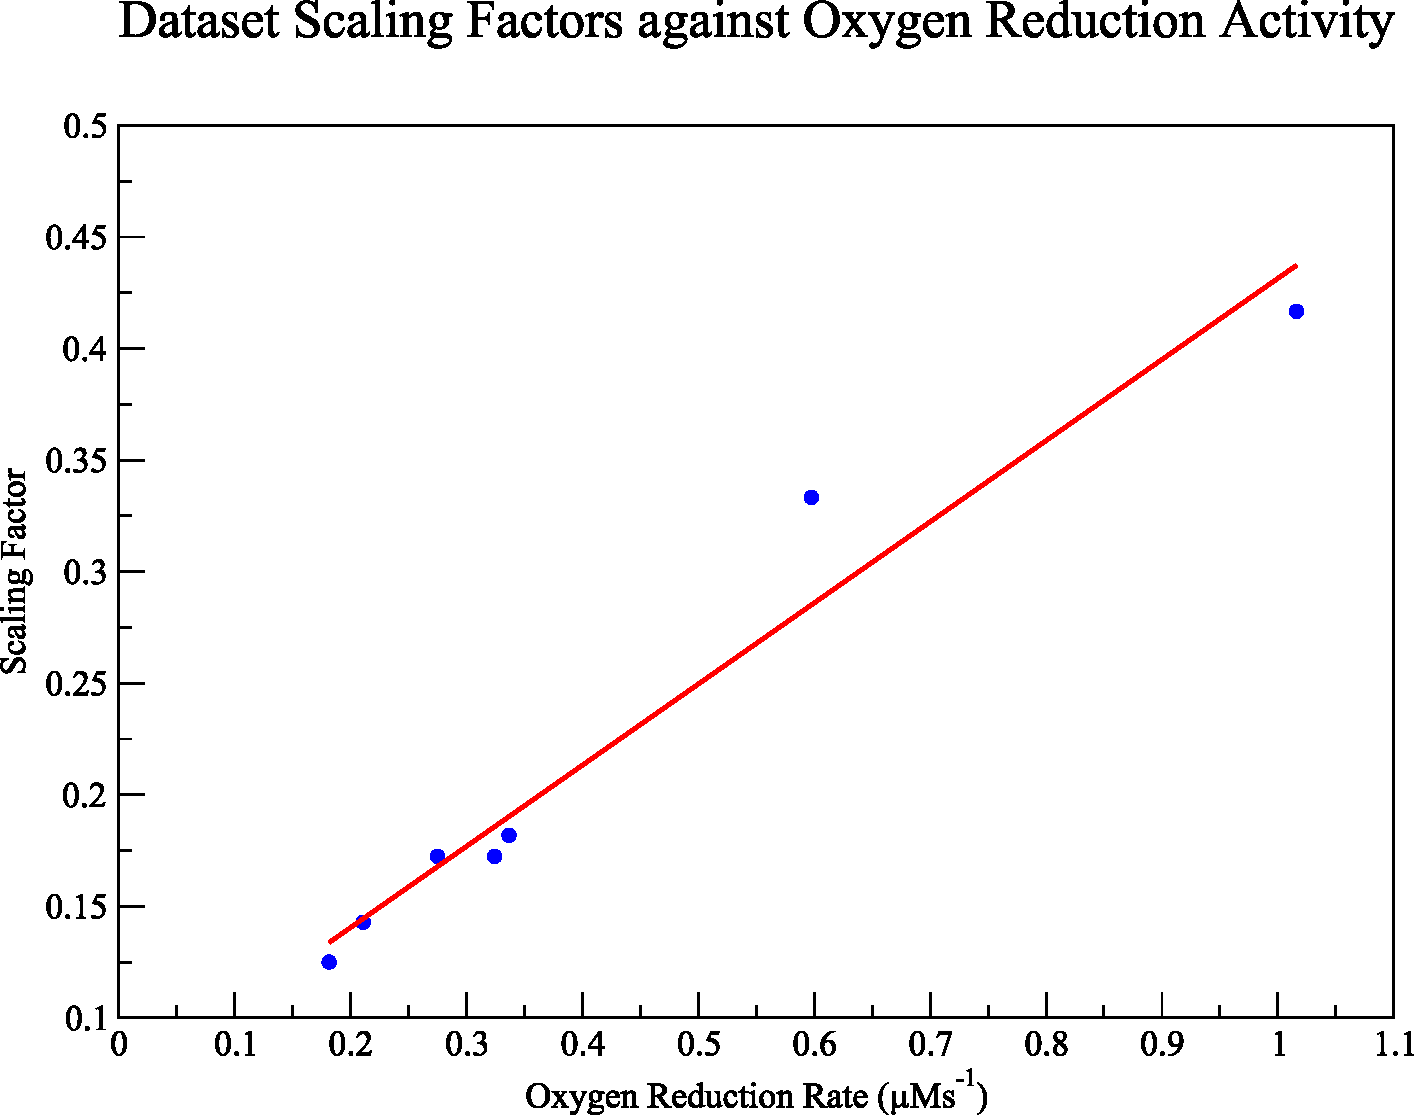
\includegraphics[width=15cm, clip=true]{./09-completedmodel/data/scaling.pdf}
 % in_silico_nsrR.pdf: 705x525 pixel, 72dpi, 24.87x18.52 cm, bb=0 0 705 525
 \caption[Dataset Scaling Factors]{{\bf Dataset Scaling Factors}. This figure shows the magnitude of the scaling factor relative to the experimental oxygen reduction rates. The red lines indicates a linear regression through the datapoints.
 \label{fig:scaling-factors}}
\end{figure}

\section{Concluding Remarks}
The parameterised model created in this work appears to be capable of at least qualitatively modelling the behaviour of all the datasets presented, using the final set of parameter distributions. The model is not 100\% quantitative, although this was not an implicit requirement for the model. It should still be capable of offering insight into how the system behaves even if it cannot predict changes precisely. The non-quantitative nature of the model was to be expected given the high level of complexity in the model and some of the assumptions made regarding cytochromes, backward reaction rates etc. The most obvious ``fault'' in the model is that there is an incomplete decoupling of cell density from other components. Unfortunately this is most probably because the proxy used was not completely accurate as a replacement for cell density.

The integrated parameter estimation system created for this work operates as intended and could be extended to parameterise other systems if the same Bayesian approach were taken to data gathering. It is not however a system that could be used without human curation though, as it can still produce mathematically correct results with parameters that are actually very unlikely \textit{in vivo}. This was shown in Chapter \ref{chap:nitritereduction} where the values for 2 parameters were an order of magnitude too high in the prior probability distributions causing the simulation to fail. These same values worked ``perfectly'' for the datasets in Chapters \ref{chap:oxygenreduction} and \ref{chap:noreduction}. Such human interaction with the system is important however as it forms part of the Bayesian approach whereby we provide the ``prior'' knowledge to the system.

In conclusion, a novel system for parametrising a respiration system model has been created and utilised which has been able to successfully populate the model and produce probability distributions for all parameters. These parameters are able to be used in a qualitative manner to match existing experimental data, and to provide insight into the hidden behaviour of the system.